
\chapter{OpenFOAM}
\rhead{OpenFOAM}
\begin{refsection}

\chapterauthor{Gregor Dengler}
\newpage
\section{Einleitung}
OpenFOAM (Open Source Field Operation and Manipulation) ist ein in C++ geschriebenes, numerisches, freies Simulationssoftwarepaket. Es wurde ursprünglich in den späten 1980er Jahren am Imperial College in London entwickelt. OpenFOAM war jedoch nicht von Anfang an Open Source, erst im Jahr 2004 nachdem es verkauft wurde, wurde es als OpenFOAM veröffentlicht. Das Ziel war ein Softwarepaket zu erstellen, welches flexibler und besser als das bis dato genutze FORTRAN (Formula Translating System) ist.\\
OpenFOAM besteht nicht nur aus den Solvern für die verschiedenen Probleme, sondern besitzt auch Pre-Processing sowie Post-Processing Tools. Im Pre-Processing wird vor allem ein Meshing Tool zur Verfügung gestellt. Im Post-Processing wird mittels ParaView eine übersichtliche Darstellung der berechneten Daten ermöglicht. \cite{wiki} 
\\
Im Pre-Processing wird die Geometrie definiert und Randbedingungen vorgegeben. Es wird also definiert, was genau simuliert werden soll. Randbedingungen sind Vorgaben zum Verhalten der Simulation am Rande des simulierten Bereichs, sowie auf Oberflächen. \\
Während des solven, dem Lösen der Strömungsdiffereitialgleichungen oder allgemein der Feldgleichungen, wird die eigentliche Berechnung von Solver ausgeführt. Solver sind Programme, welche die Algorithmen von OpenFOAM zur Lösung von partitiellen Differenzialgleichungen beinhalten.  \\
Das Post-Processing soll die Berechnung visualisiert werden. Des Weiteren können im Post-Processing auch physikalisch relevante Grössen aus der Berechnung extrahiert werden. \\
\begin{minipage}{\linewidth}
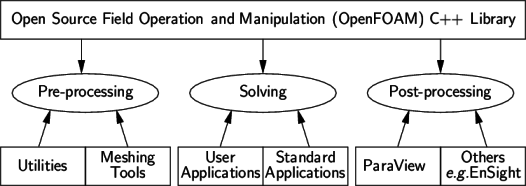
\includegraphics[width = 0.65 \linewidth]{./OpenFOAM/Pics/Aufbau.png}
\captionof{figure}{OpenFOAM im Überblick \cite{of}
}
\end{minipage}
\section{Einsatzgebiete von OpenFoam}
Es gibt in OpenFOAM eine ganze Reihe verschiedener Standard Solver für diverse Probleme. Hier eine kleine Übersicht, für welche Bereiche es bereits Standard Solver gibt:
\setlist{nolistsep}
\begin{itemize}
\setlength{\itemsep}{2pt}
\setlength{\parsep}{2pt}
\item Basic CFD codes  
\item Incompressible flow 
\begin{itemize}
\item \textbf{icoFoam}
\item \textbf{pisoFoam}
\end{itemize}
\item Compressible flow 
\item Multiphase flow
\item Direct numerical simulation (DNS) and large eddy simulation (LES)
\item Combustion
\item Particle-tracking flows
\item Heat transfer and buoyancy-driven flows
\item Molecular dynamics methods
\item Direct simulation Monte Carlo methods
\item Electromagnetics
\item Stress analysis of solids
\item Finance
\end{itemize} 

Da OpenFOAM Open Source ist und zudem sehr flexibel, wird es häufig in der Forschung eingesetzt. Der Vorteil liegt darin, dass nicht nur der Solver an sich, sondern auch die konkrete nummerischen Lösungsverfahren für die verschiedenen Gleichungen leicht eingestellt werden können. Man hat zudem die Möglichkeit, sich nebst den Standard Solvern auch Eigene zu erstellen. So lässt sich OpenFOAM mit einem gewissen Aufwand auf jedes Problem zuschneiden. \cite{of} 

\section{Beispiel Cavity}
\subsection{Pre-Processing}
Ich habe mit dem Tutorial Beispiel Cavity und dem Solver IcoFOAM begonnen. Im Beispiel Cavity geht es um die Simulation einer Strömung, die entsteht, wenn oberhalb einer offenen Box ein Luftzug durchweht. Es interessiert also in diesem Beispiel lediglich, was innerhalb der Box geschieht. Grundsätzlich muss beim Beispiel Cavity nichts mehr gemacht werden, es ist bereits alles voreingestellt. Man sieht gut wie ein OpenFOAM Projekt aufgebaut sein sollte. Zudem lässt sich der Einfluss der Anzahl Zellen und der Simulationszeit einfach veranschaulichen. \\
\begin{minipage}{0.5 \linewidth}
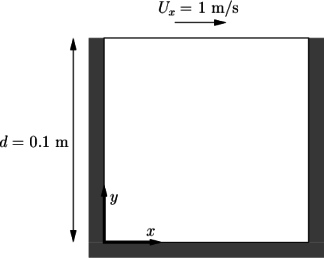
\includegraphics[width =  \linewidth]{./OpenFOAM/Pics/cavity1.png} 
\captionof{figure}{Beispiel Cavity %\cite{of} 
}
\end{minipage} 
\\
\begin{minipage}{0.5 \linewidth}
Im Bild nebenan sieht man die Ordnerstruktur eines OpenFOAM Projekts. In den verschiedenen Files lassen sich verschiedene Parameter einstellen. \\
Im Ordner  \texttt{System} ist alles grundsätzliche definiert. So wird im File  \texttt{controlDict} festgelegt, welcher Solver verwendet werden soll, hier z.B. icoFOAM. Dann wird der Start sowie das Ende der Simulation definiert. In diesem Beispiel wird eine Startzeit von 0 s festgelegt und eine Endzeit von 0.5 s. Des Weiteren werden die Zeitschritte festgelegt, hier 0,005 s. Es werden noch weitere Parameter eingestellt, wie Ausgabeformat usw. \\
Im File  \texttt{fvSchemes} wird vorgegeben, welche nummerischen Lösungsverfahren zur Lösung der Gleichungen verwendet werden sollen.\\
Im File \texttt{fvSolution} wird für jede Art Gleichung eine Lösungsalgorithmus bestimmt.  Hier stehen Algorithmen zur Auswahl, die in früheren Kapiteln dieses Buchs erläutert wurden. So z.B. Der Gauss-Seidel Algorithmus.\\
\end{minipage}
\begin{minipage}{0.5 \linewidth}
\hspace{0.5cm}
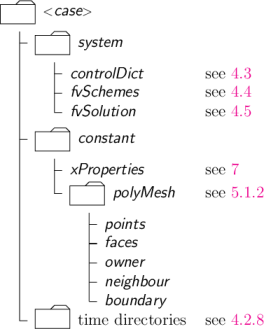
\includegraphics[width =  \linewidth]{./OpenFOAM/Pics/Struktur.png}
\captionof{figure}{Ordnerstrucktur eines OpenFOAM Projekts % \cite{of}
}
\end{minipage}
\begin{minipage}{\linewidth}
 Im Ordner  \texttt{constant} wird vor allem die Form des zu simulierenden Gegenstands bestimmt. Das Ganze geschieht mit dem Tool blockMesh. Um es zu nutzen, muss zuerst in einem Text-File jeder Punkt der benötigt wird mit seinen X-Y-Z Koordinaten bestimmt werden. In diesem Fall muss nur ein Block erstellt werden, d. h. insgesamt 8 Punkte. 
 \\
\end{minipage}
 \begin{minipage}{0.5 \linewidth}
Nebenan sieht man Auszüge aus dem File \texttt{blockMeshDict}. Unter \texttt{vertices} sind die erwähnten 8 Punkte definiert. Da man hier eine eigentlich 2 dimensionale Simulation machen will und Effekte der dritten Dimension nicht interessieren, sind die Punkte in der dritten Dimension sehr nahe bei einander. OpenFOAM kann keine 2D Simulationen, also muss man sich hier selbst etwas zu helfen wissen. 
\end{minipage}
\begin{minipage}{0.5 \linewidth}
\hspace{0.5 cm}
\includegraphics[width = 0.5 \linewidth]{./OpenFOAM/Pics/Punkte.png}
\captionof{figure}{Codebeispiel Cavity}
\end{minipage}
\begin{minipage}{0.5 \linewidth}
In der zweiten Abbildung sieht man unter blocks, wie so ein Block definiert wird. In der ersten Klammer sind die Punkte, welche den Block begrenzen. Hier ist es wichtig die Reihenfolge der Punkte zu beachten. Die Zahl entspricht der unter \texttt{vertices} genanten Punkte in der Reihenfolge, in der sie genant werden. 
\end{minipage}
\begin{minipage}{0.5 \linewidth}
\hspace{0.5 cm}
\includegraphics[width =  \linewidth]{./OpenFOAM/Pics/Blocks.png}
\captionof{figure}{Codebeispiel Cavity}
\end{minipage}
\begin{minipage}{0.5 \linewidth}
Definiert man seine Blocks in der falschen Reihenfolge, so verändert man die Form der Blocks. Da \texttt{blockMesh} die Linie, welche den Block begrenzt genau der Reihenfolge nach zieht, in der die Punkte in der Klammer genannt werden. In der zweiten Klammer defniert man, wieviele Zellen in welcher Dimension angelegt werden sollen.  Hier sind das 20 in X sowie Y Richtung und 1 in Z Richtung. Dies weil es eigentlich eine 2D Simulation werden soll. \\
In der Abbildung nebenan sieht man, wie die verschiedenen \texttt{Walls} definiert werden. Auch hier sind in den Klammern die Punkte, welche die Wall definieren aus\texttt{vertices} genannt. In dieser Simulation gibt es 3 Typen von Walls, die \texttt{movingWalls}, die \texttt{fixedWalls} und  \texttt{frontAndBack}. Unter \texttt{movingWalls} ist die Wand, welche für uns am interessantesten ist, da sie den offenen Teil der Box darstellt. Hier soll die Strömung durchfliessen. Die \texttt{fixedWalls} sind die Wände der Box, die simuliert werden soll. Unter \texttt{frontAndBack} sind die beiden Walls gemeint, welche die Front- und Rückansicht darstellen und auf diese Simulation keinen Einfluss haben sollen. Deshalb sind diese Walls als \texttt{empty} definiert.\\
\end{minipage}
\begin{minipage}{0.5 \linewidth}
\hspace{0.5 cm}
\includegraphics[width = 0.5 \linewidth]{./OpenFOAM/Pics/Walls.png}
\captionof{figure}{Codebeispiel Cavity}
\end{minipage}
\\
\texttt{Time directories} ist ein Überbegriff für eine ganze Reihe von Ordnern. Wenn man keine Veränderungen der grundsätzlichen Situation während der zu simulierenden Zeit machen will, muss man lediglich einen Ordner  \texttt{0} erstellen. In diesem Ordner wird alles definiert, was während der Simulation nicht ändert. Im Beispiel Cavity sind die Variablen  \texttt{p} und  \texttt{U} vordefiniert. Im File p wird der Anfangsdruck und im File U die Anfangsgeschwindigkeit bestimmt. Wenn man nun noch eine Veränderung während der Simulation erreichen will, so müsste man das entsprechende Verzeichnis erstellen und die Veränderung darin definieren. 
 \subsection{Berechnung}
 Sind nun alle Voreinstellungen gemacht, lässt sich die Berechnung mittels Befehl icoFOAM starten. Alternativ kann man mit OpenMPI auch eine parallele Berechnung auf mehreren Prozessoren durchführen. Dafür wird eine kleine Vorbereitung benötigt. Es muss in einem weiteren Textfile namens \texttt{decomposeParDict} definiert werden, auf wie viele Prozessoren die Arbeit verteilt werden soll. Des Weiteren muss man definieren wie die Arbeit aufgeteilt wird. So kann man angeben, wie viele Unterteilungen es in jeder Dimension geben soll. Ein weiter Punkt, der definiert wird, ist die, wie sehr der Rechenaufwand pro Prozessor voneinander abweichen darf. Danach wird das \texttt{decomposePar} gestartet und der Computer erstellt für jeden Prozessor ein eigenes Verzeichnis. Nun ist die Arbeit fertig aufgeteilt. Jetzt kann man die Simulation starten. Das wird mit dem Befehl \texttt{mpirun -np 16 icoFoam -parallel} gemacht. Hier ist wichtig, dass der Funktion icoFoam die Option parallel mit übergeben wird, da sonst trotz Vorbereitung nur auf einem Prozessor gerechnet wird.\\
 Ist die Berechnung abgeschlossen, muss man im Falle der parallelen Berechnung die Daten der verschiedenen Prozessoren wieder zusammenfügen. Dies geschieht mit dem Befehl \texttt{reconstructPar}. Dieser Befehl macht aus den verschiedenen Verzeichnissen der verschiedenen Prozessoren wieder ein Verzeichnis in dem alle Ergebnisse sind. Erst dann lassen sie sich mittels ParaFOAM visualisieren. 
\subsection{Post-Processing}
Sind die Daten nach dem parallelen Berechnen wieder richtig zusammengefügt, so lassen sich diese nun mit dem Befehl paraFoam anschauen. Es wird nun paraView geöffnet und man kann sich die verschiedenen Daten anzeigen lassen. \\ \\
\begin{minipage}{0.5 \linewidth}
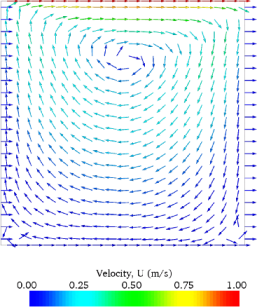
\includegraphics[width = 0.8 \linewidth]{./OpenFOAM/Pics/stroemung.png}
\captionof{figure}{Cavity Vektoransicht %\cite{of}
}
\end{minipage}
\begin{minipage}{0.5 \linewidth}
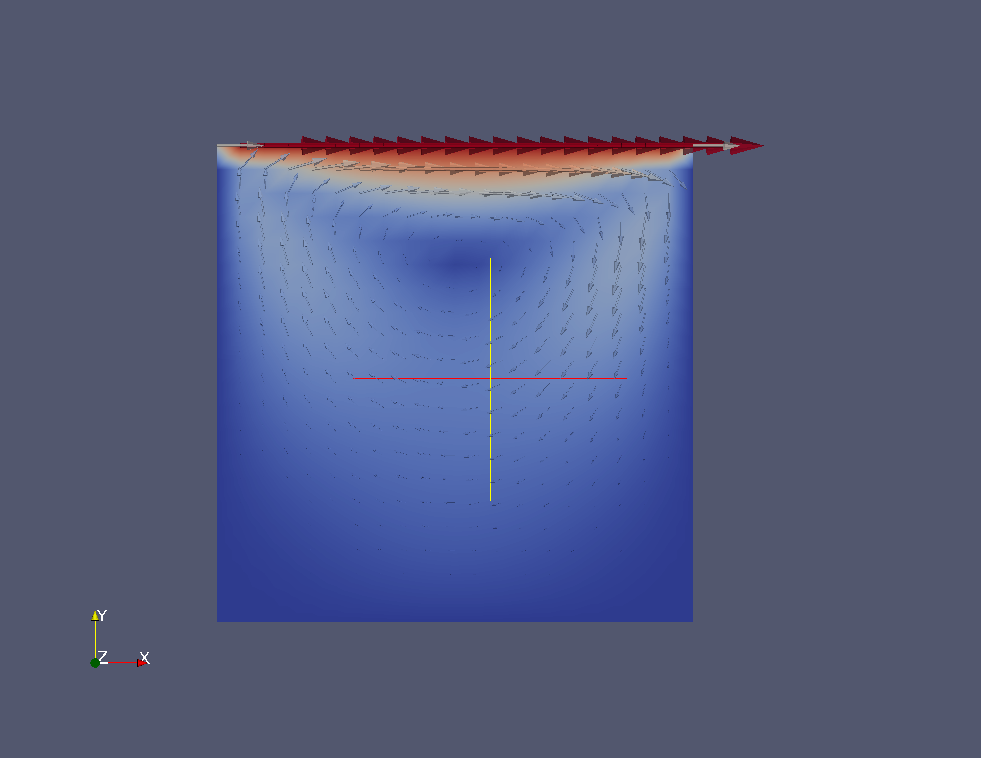
\includegraphics[width = \linewidth]{./OpenFOAM/Pics/stroemung2.png}
\captionof{figure}{Cavity Strömungsansicht %\cite{of}
}
\end{minipage} \\
Auf diesen Bildern ist die Strömung innerhalb der Box sehr gut zu erkennen. Es bildet sich innerhalb der Box ein Wirbel, wie man das von Anfang an erwartet hat. Es lässt sich in ParaView aber nicht nur der Schlusszeitpunkt anschauen. Man kann auch den Verlauf der Strömung in einer Art Video ansehen.
\section{Beispiel Keil}
Das Beispiel Keil habe ich selber versucht mit Cavity als Grundlage zu erarbeiten. Im Grundsatz geht es um einen Keil, der in einem Windkanal in einer Strömung steht. In diesem Beispiel erwarte ich, dass sich hinter dem Keil ein grösserer Wirbel bilden wird. Um nun in diesem intressanten Bereich genug Daten zu sammeln empfiehlt es sich, in diesem Bereich etwas mehr Zellen zu generieren. Dafür muss der Raum hinter dem Keil in mehrere Blöcke eingeteilt werden.
\subsection{Mesh}
In diesem Beispiel hab ich, nach anfangs gescheitertem Versuch mit gmsh, mit dem blockMesh von OpenFoam gearbeitet. Wie schon erwähnt, habe ich hierfür alle Punkte von Hand in ein Textfile geschrieben. In diesem Beispiel bedeutet das 174 Punkte. Zusätzlich muss man noch alle Blöcke als solche definieren, hier 23. Als Letztes werden alle Aussenflächen definiert, hier waren das 65 Flächen.\\
 Mit den hier definierten Blocks unterteilt man die Berechnung. Man kann so an interessanten Stellen mehr Zellen erzeugen und an weniger interessanten Stellen weniger. Sind 2 Blöcke direkt benachbart, so erkennt das OpenFOAM. Hierfür ist es aber notwendig, dass die Punkte in richtiger Reihenfolge eingegeben wurden. Für alle Blocke die am Rand sind, muss für die aussenliegenden Flächen definiert werden, was sie für einen Einfluss auf die Simulation haben. In dieser Simulation sind das alle Flächen oben und unten sowie an den Seiten des Windkanals die keinen Einfluss haben sollen und die Fläche vorne und hinten welch offen sein sollen. Die Flächen des Keils selber sollen sich wie fixe Wände verhalten. \\
\begin{minipage}{\linewidth}
\centering
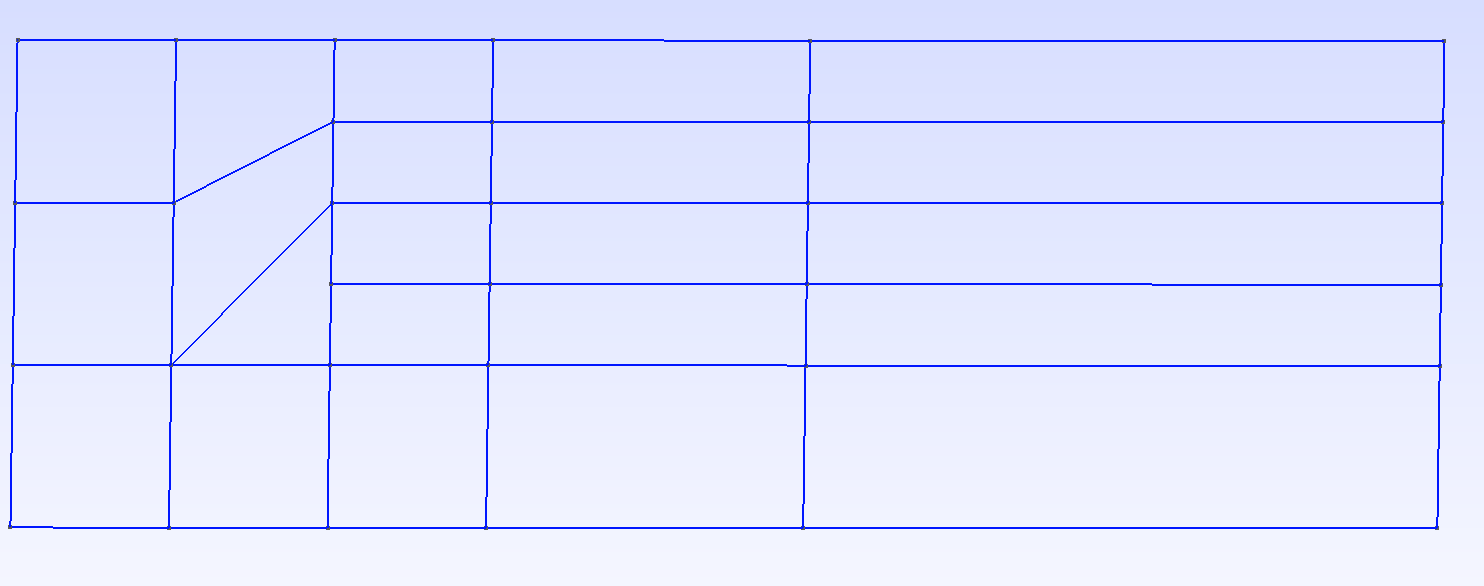
\includegraphics[scale = 0.1]{./OpenFOAM/Pics/Keil.png} \captionof{figure}{Mesh Mit gmsh}
\end{minipage}
 \\
Wie gut zu erkennen ist, ist der Keil ganz am Anfang des Windkanals. Das, weil die interessanten Wirbel vor allem nach dem Keil entstehen werden und man so genug davon sehen kann. Auch gut zu erkennen ist, dass ich die Blöcke in unmittelbarer Nähe zum Keil sehr klein gewählt habe. Dies hab ich so gewählt, weil ich in jedem Block gleich viele Zellen definiert habe. Man hat also rund um den Keil viel mehr und viel kleinere Zellen als gegen Schluss des Windkanals. Ich habe in diesem Beispiel 200 x 200 Zellen pro Block gewählt, also 23 x 200 x 200 (=920'00)Zellen.
\subsection{Die Courant-Zahl}
Will man mit einer CFD (Computational Fluid Dynamics) Software etwas berechnen, so hat man bei den Einstellungen zu beachten, dass die Berechnung stabil bleibt. Um dies zu erreichen, muss die sogenannte Courant-Zahl (auch Courant-Friedrichs-Lewy-Zahl genannt) zwingend unter 1 bleiben. \\ \\
$c = \frac{u \cdot \Delta t}{\Delta x} < 1$ 
\\ \\
In meiner Simulation ist die höchste auftretende Geschwindigkeit $u$ die Schallgeschwindigkeit. Die grösste Ortschritt $\Delta x$ wird durch die Zellengrösse definiert. Will man eine erfolgreiche Simulation durchführen, muss man den Zeitschritt klein genug wählen. Das Problem mit kleinen Zeitschritten ist, dass man sehr viel Rechenaufwand hat, wählt man ihn aber zu gross so bricht die Simulation eventuell nach einiger Zeit ab. 
Bei der Simulation vom Keil wurde ein Zeitschritt von 0,1 ms gewählt um diese Bedingung zu erfüllen.

\subsection{Berechnung}
Die Berechnung vom Beispiel Keil wurde auf 32 Cores gestartet. Insgesamt wurde während ca 6 Tagen auf allen 32 Cores mit Vollast gerechnet. In dieser Zeit konnten 0.67 s der Simulation berechnet werden. Dass entspricht ca 6,2 Mia. Berechnungen. In dieser Zeit wurden 8,7 GB Daten generiert. Wie schon die etwas ungewöhnliche Simulationszeit erahnen lässt, war ursprünglich nicht geplant, nur 0.67 s zu simulieren. Es ist jedoch nach 0.67 s zu einem Überschreiten der Courant-Zahl und somit zum Abbruch wegen Divergenz gekommen. Dies, weil die Druckänderung an der Anfangspitze des Keil zu gross wurde und sie somit die Zellengrösse übersprang. 

\subsection{Ergebnis}
Das Ergebnis lässt sich mittels ParaView visualisieren. Man merkt beim Begutachten der Resultate mit ParaView schnell, dass es sich um sehr viele Daten handelt, da es sehr langsam läuft. Das Ergebnis ist aber so herausgekommen wie im Voraus erwartet. Es löst sich, wie anfangs angenommen, an der oberen Spitze des Keils ein Wirbel ab. Was etwas extremer ausfällt als erwartet, ist die Kompression am Anfang des Keils. An dieser Stelle entsteht ein sehr hoher Druck, was auch zum Abbruch der Simulation geführt hat. \\
\begin{minipage}{0.5 \linewidth}
\includegraphics[width = \linewidth]{./OpenFOAM/pics/u1.png}
\end{minipage}
\begin{minipage}{0.5 \linewidth}
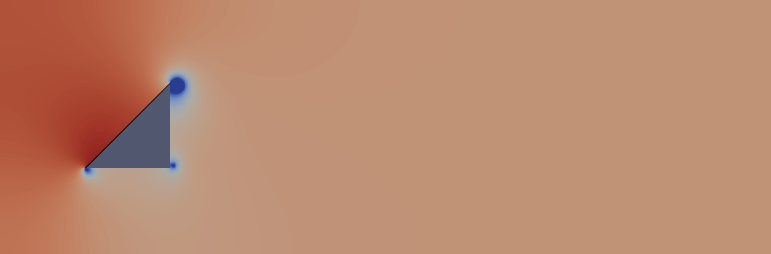
\includegraphics[width = \linewidth]{./OpenFOAM/pics/p1.png}
\end{minipage} \\
\begin{minipage}{0.5 \linewidth}
\includegraphics[width = \linewidth]{./OpenFOAM/pics/u5.png}
\end{minipage}
\begin{minipage}{0.5 \linewidth}
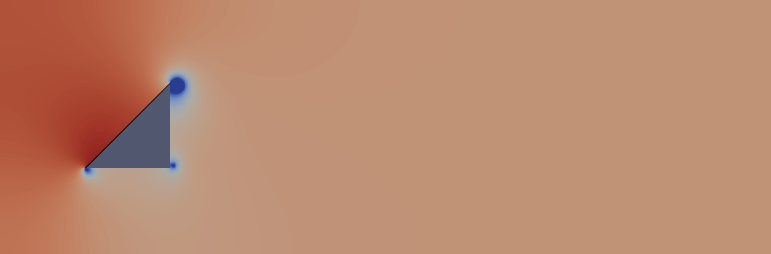
\includegraphics[width = \linewidth]{./OpenFOAM/pics/p1.png}
\end{minipage}\\
\begin{minipage}{0.5 \linewidth}
\includegraphics[width = \linewidth]{./OpenFOAM/pics/u25.png}
\end{minipage}
\begin{minipage}{0.5 \linewidth}
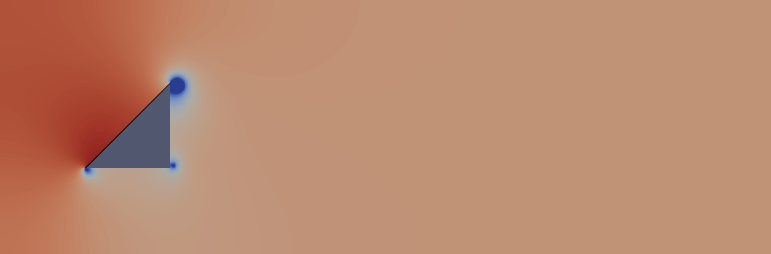
\includegraphics[width = \linewidth]{./OpenFOAM/pics/p1.png}
\end{minipage}\\
\begin{minipage}{0.5 \linewidth}
\includegraphics[width = \linewidth]{./OpenFOAM/pics/u55.png}
\captionof{figure}{Bilder der Strömung nach 10, 50, 250, 550 ms}
\end{minipage}
\begin{minipage}{0.5 \linewidth}
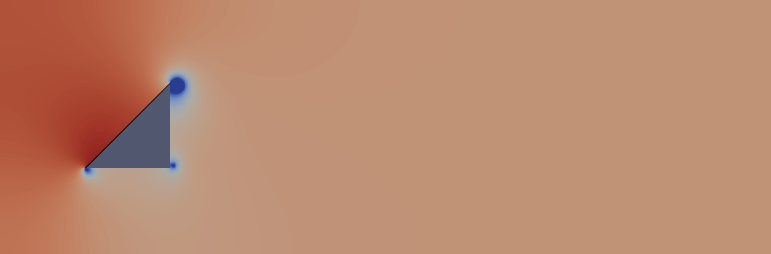
\includegraphics[width = \linewidth]{./OpenFOAM/pics/p1.png}
\captionof{figure}{Bilder des Drucks nach 10, 50, 250, 550 ms}
\end{minipage}


\section{Probleme}
Ich hatte während der Arbeit mit OpenFOAM mit Problemen zu kämpfen. In diesem Abschnitt wird beschrieben, wo ich am meisten Zeit verloren habe und wie man sich diesen Ärger sparen kann.
\subsection{Installation}
Während meiner Arbeit mit OpenFOAM kostete alleine schon die Installation sehr viel Zeit. Dies, weil ich den Fehler machte, eine nicht voll kompatible OpenSuse Version zu verwenden. Das führte dazu, das ich das vorbereitete Package nicht gebrauchen konnte und mir das Softwarepaket aus dem Sourcecode selbst kompilieren musste. \\
Hierfür wurden diverse zusätzlichen Packages benötigt, welche ich selber korrekt installieren musste. Für mich als Linux-Anfänger war das nicht immer ganz einfach und ich musste mich oft auf Hilfe von Mitbewohnern und Mitstudenten berufen. Schlussendlich brachte ich das Softwarepaket fast zum Laufen. Das Einzige, was unter Linux nie funktionierte, war die Visualisierung mit ParaView. Hier gab es ein Problem mit der Software Paralles, welche die virtuelle Maschine, in der Linux läuft, betreibt. \\
Ich versuchte, das ganze unter Mac OS X zum Laufen zu bringen. Auch hier mit bescheidenem Erfolg. Das einzige, was korrekt installiert wurde unter Mac OS X war ParaView. Somit konnte ich die Berechnungen unter Linux bzw. mittels HPC der HSR berechnen lassen und mit ParaView unter Mac OS X visualisieren.\\
 Beim nächsten Mal würde ich nicht mehr versuchen, OpenFOAM in einer virtuellen Maschine zu installieren, sondern auf einem Computer mit nativ Linux. Dies hätte mir viel Arbeit erspart.

\subsection{BlockMesh}
Mein zweites grosses Problem war, dass ich zwar versuchte, mit gmsh ein Mesh meiner Simulation zu erstellen, dies aber am Einbinden ins OpenFOAM scheiterte. Hier ist zu erwähnen, dass ich aufgrund der verlorenen Zeit bei der Installation nicht alle Möglichkeiten ausgeschöpft habe, sondern ziemlich schnell entschied, mit BlockMesh und der Eingabe von Hand ins Textfile mein Mesh zu erstellen. \\
Das Hauptproblem beim Blockmesh ist, dass man auch nach dem meshen das Ergebnis nicht visualisieren kann, es benötigt also eine sehr sorgfältige Eingabe der verschiedenen Punkte und Blocks. Hier hatte ich in einem meiner 174 Punkte in einer Dimension einen Tippfehler, welchen ich selber nicht finden konnte. Herr Müller entdeckte diesen beim Untersuch meiner Probleme. \\ Danach konnte die Simulation, nach Behebung weiterer kleiner Ungereimtheiten und nach fertigem Erstellen der Files fvScheme und fvSolution, gestartet werden. Wie schon erwähnt brach dann die Simulation nach 0.67 s Simulationszeit ab. Dies war aber nicht weiter tragisch, da Herr Müller am Abend, als es zum Abbruch kam, die Simulation sowieso abbrechen wollte um die Ergebnisse für die Vorlesung Numb3rs @ HSR zu verwenden.

\section{Fazit}
Mein persönliches Fazit zur Arbeit mit OpenFOAM fällt nicht besonders positiv aus, da es sehr aufwändig ist, sich in OpenFOAM einzuarbeiten. Ich bin mir aber sicher, dass wenn man das Softwarepaket einmal im Griff hat, man seine Ziele auch innert nützlicher Frist erreichen kann. Ich kann mir gut vorstellen, dass sich mit einigem Training und genügend einarbeiten in dieses Softwarepaket auch komplexe Probleme lösen lassen. Der grosse Vorteil von OpenFOAM gegenüber den kommerziellen Lösungen, wie z.B. COMSOL Multiphysics, welches z.B. im Modul angewandter Elektromagnetismus Felder und Wellen eingesetzt wird, ist, dass es Open Source ist und somit beliebig parallelisiert werden kann, ohne für jeden Thread eine Lizenz erwerben zu müssen. Kommerzielle Softwarelösungen, welche einen solch breiten Bereich abdecken, sind in der Regel sehr teuer und somit lässt sich mit OpenFOAM sehr viel Geld einsparen. Ein weiterer Vorteil von Open Source Software ist, dass man genau weiss, was und wie gerechnet wird. Es lassen sich auch eigene Solver schreiben, wenn man z. B. ein Problem hat, für das es noch keinen gibt. Dies wiederum macht die Software sehr flexibel. Die Tatsache, dass man jedes Lösungsverfahren selber definieren kann, macht die Software noch flexibler. Hier kommt allerdings auch einer der grossen Nachteile zum Tragen. Man muss genau wissen, was man macht, da man sonst nicht auf ein gewünschtes Resultat kommt. \\
Es gibt für OpenFOAM sehr viele Forumbeiträge, in denen diverse Probleme gelöst und erklärt werden, jedoch ist es für Anfänger etwas schwierig, da nicht alles sauber dokumentiert ist und man nicht immer versteht, wie man gewisse Einstellungen richtig nutzt. 
\printbibliography[heading=subbibliography]
\end{refsection}